%==========================================================================================================
% MULAI BAB II
%==========================================================================================================
\chapter{DASAR TEORI}
\label{chap:dasar_teori}
%==========================================================================================================
% Subbab
%==========================================================================================================

\section{\textit{Augmented Reality}}
\label{sec:AR}
\textit{Augmented reality} (AR) adalah sebuah istilah untuk lingkungan yang menggabungkan dunia nyata dan dunia virtual yang dibuat oleh komputer sehingga batas antara keduanya menjadi sangat tipis. Ronald Azuma pada tahun 1997 \cite{Azuma1997} mendefinisikan \textit{Augmented Reality} sebagai sistem yang memiliki karakteristik sebagai berikut:
\begin{itemize}
	\item Menggabungkan lingkungan nyata dan virtual
	\item Berjalan secara interaktif dalam waktu nyata
	\item Integrasi dalam tiga dimensi (3D)
\end{itemize}
Secara sederhana AR bisa didefinisikan sebagai lingkungan nyata yang ditambahkan objek virtual. Penggabungan objek nyata dan virtual dimungkinkan dengan teknologi \textit{display} yang sesuai, interaktivitas dimungkinkan melalui perangkat-perangkat input tertentu.  

AR merupakan variasi dari \textit{Virtual Environments} (VE), atau yang lebih dikenal dengan istilah \textit{Virtual Reality} (VR). Teknologi VE membuat pengguna tergabung dalam sebuah lingkungan virtual secara keseluruhan. Ketika tergabung dalam lingkungan tersebut, pengguna tidak bisa melihat lingkungan nyata di sekitarnya. Sebaliknya, AR memungkinkan pengguna untuk melihat lingkungan nyata, dengan objek virtual yang ditambahkan atau tergabung dengan lingkungan nyata. Tidak seperti VR yang sepenuhnya menggantikan lingkungan nyata, AR sekedar menambahkan atau melengkapi lingkungan nyata \cite{Azuma1997}. 

Tujuan utama dari AR adalah untuk menciptakan lingkungan baru dengan menggabungkan interaktivitas lingkungan nyata dan virtual sehingga pengguna merasa bahwa lingkungan yang diciptakan adalah nyata. Dengan kata lain, pengguna merasa tidak ada perbedaan yang dirasakan antara AR dengan apa yang mereka lihat/rasakan di lingkungan nyata. Dengan bantuan teknologi AR (seperti visi komputasi dan pengenalan objek) lingkungan nyata disekitar kita akan dapat berinteraksi dalam bentuk digital (virtual). Informasi tentang objek dan lingkungan disekitar kita dapat ditambahkan kedalam sistem AR yang kemudian informasi tersebut ditampilkan diatas \textit{layer} dunia nyata secara \textit{real-time} seolah-olah informasi tersebut adalah nyata. Informasi yang ditampilkan oleh objek virtual membantu pengguna melaksanakan kegiatan-kegiatan dalam dunia nyata. AR banyak digunakan dalam bidang-bidang seperti kesehatan, militer, industri manufaktur dan juga telah diaplikasikan dalam perangkat-perangkat yang digunakan orang banyak, seperti pada telepon genggam. 

\section{\textit{Mixed Reality}}
\label{sec:mixed_reality}
Paul Milgram and Fumio Kishino merumuskan  kerangka kemungkinan penggabungan dan peleburan dunia nyata dan dunia maya yang disebut \textit{\textbf{Milgram's Reality-Virtuality Continuum}} pada tahun  1994.  Dalam Gambar \ref{fig:milgram_continuum}, sisi yang paling kiri adalah lingkungan nyata yang hanya berisi benda nyata, dan sisi paling kanan adalah lingkungan maya yang berisi benda maya \cite{Milgram1994a}.  

\begin{figure}[h]
\begin{center}
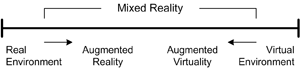
\includegraphics{./images/Milgram_Continuum}
\caption{\label{fig:milgram_continuum} Mixed Reality}
\end{center}
\end{figure}

Dalam \textit{augmented reality}, yang lebih dekat ke sisi kiri, lingkungan bersifat nyata dan benda bersifat maya, sementara dalam \textit{augmented virtuality}, yang lebih dekat ke sisi kanan, lingkungan bersifat maya dan benda bersifat nyata. 

\section{\textit{Komponen \textit{Augmented Reality}}}
\label{sec:komponen_ar}

\section{Teknik Display \textit{Augmented Reality}}
\label{sec:AR_display}
Sistem \textit{display} AR merupakan sistem manipulasi citra yang menggunakan seperangkat optik, elektronik, dan komponen mekanik untuk membentuk citra dalam jalur optik antara mata pengamat dan objek fisik yang akan digabungkan dengan teknik AR. Bergantung kepada optik yang digunakan, citra bisa dibentuk pada sebuah benda datar atau suatu bentuk permukaan yang kompleks (tidak datar)\cite{Bimber2005}. Gambar \ref{fig:diagram_display_AR} mengilustrasikan kemungkinan citra akan dibentuk untuk mendukung AR, peletakan display bergantung dari pandangan pengguna dan objek, dan tipe citra seperti apa yang akan dihasilkan (\textit{planar} atau \textit{curved}).

\begin{figure}[h]
	\begin{center}
	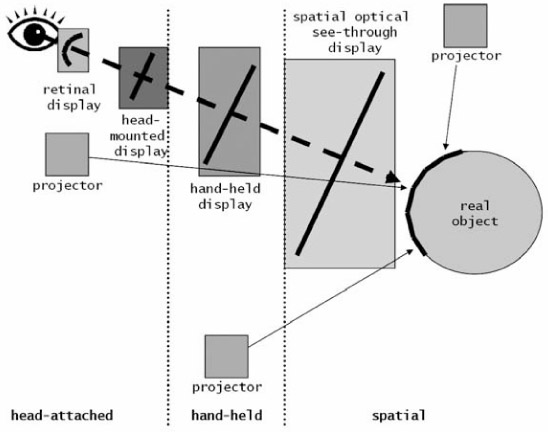
\includegraphics[width=10cm]{images/diagram_display_AR}
	\caption{\label{fig:diagram_display_AR}Pembentukan citra untuk display \textit{augmented reality}}
	\end{center}
\end{figure}

Secara garis besarnya ada tiga teknik display AR \cite{Bimber2005}, yaitu sebagai berikut:

\begin{enumerate}
\item \textit{Head-Attached Display}
\item \textit{Handheld Display}
\item \textit{Spatial Display}
\end{enumerate}

\subsection {\textit{Head-Attached Display}}
\label{subsec:HAD}
\textit{Head-Attached Display} merupakan teknik display yang mengharuskan penggunanya untuk memakai sistem ini di kepala pengguna. Berdasarkan teknik citra yang terbentuk, \textit{Head-Attached Display} terbagi tiga, yaitu sebagai berikut: 
\begin{itemize}
\item \textit{Head-Mounted Display}. 
\item \textit{Head-Mounted Projectors}.
\item \textit{Virtual Retina Display}. 
\end{itemize}
Kelebihan teknik display \textit{Head-Attached Display} ini adalah lebih nyaman ke pengguna, karena citra yang terbentuk mengikuti sudut pandang pengguna.

\subsubsection {\textit{Head-Mounted Display}}
\label{subsubsec:HMD}
\textit{Head-Mounted Display} (HMD) menggabungkan citra dari objek virtual dan objek nyata dan menampilkannya langsung ke mata pengguna melalui suatu alat yang dipasang di kepala pengguna. Terdapat dua tipe utama perangkat HMD yang digunakan dalam aplikasi realitas tertambah, yaitu \textit{optical-see-through} HMD dan \textit{video see-through} HMD. Keduanya digunakan untuk berbagai jenis pekerjaan dan memiliki keuntungan dan kerugian masing-masing. Dengan \textit{optical-see-through} HMD, lingkungan nyata dilihat melalui cermin semi transparan yang diletakkan di depan mata pengguna. Cermin tersebut juga digunakan untuk merefleksikan citra yang dibentuk oleh komputer ke mata pengguna, menggabungkan lingkungan nyata dan virtual. Dengan \textit{video see-through} HMD, lingkungan nyata direkam mengunakan dua kamera video yang terintegrasi ke alat, seperti gambar \ref{fig:actual_see_trough_HMD}, dan citra yang dibentuk komputer digabung dengan video tadi untuk merepresentasikan lingkungan yang akan dilihat pengguna \cite{Rolland1994}.

\begin{itemize}
\item {\textit{Video-see-through Head-Mounted Display}}

\begin{figure}[h]
\begin{center}
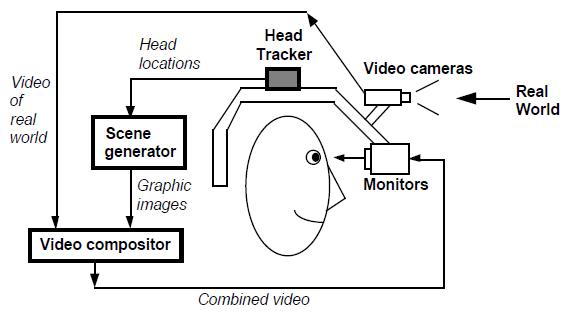
\includegraphics[width=11cm]{./images/opaque_HMD}
\caption{\label{fig:opaque_HMD} Diagram \textit{Opaque} HMD}
\end{center}
\end{figure}

\textit{Video see-through} HMD bekerja dengan menggabungkan sebuah \textit{closed-view} HMD dengan satu atau dua \textsl{head-mounted} kamera video, melalui kamera video tersebut pengguna melihat ke lingkungan nyata. Video dari kamera dikombinasikan dengan citra yang dibuat oleh \textit{scene generator}, dunia nyata dan virtual digabungkan. Hasilnya dikirimkan ke monitor yang terletak di depan mata pengguna. Gambar \ref{fig:opaque_HMD} menunjukkan konsep dari \textit{Video see-through} HMD, gambar \ref{fig:actual_opaque_HMD} adalah contoh \textit{Video see-through} HMD, dengan dua video terintegrasi di bagian atas Helm \cite{Azuma1997}.

\begin{figure}[h]
\begin{center}
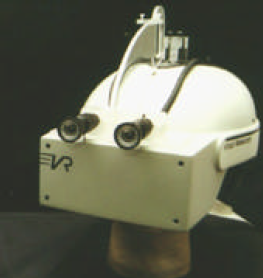
\includegraphics[width=5cm]{./images/actual_opaque_HMD}
\caption {\label{fig:actual_opaque_HMD} Contoh \textit{Opaque} HMD}
\end{center}
\end{figure}

\item {\textit{Optical see-through Head-Mounted Display}}

Tidak seperti penggunaan \textit{video see-through} HMD, \textit{optical see-through} HMD  menyerap cahaya dari lingkungan luar, sehingga memungkinkan pengguna untuk secara langsung mengamati dunia nyata dengan mata (gambar \ref{fig:see-trough_HMD}). Selain itu, sebuah sistem cermin yang diletakkan di depan mata pengguna memantulkan cahaya dari pencitraan grafis yang dihasilkan komputer. Pencitraan yang dihasilkan merupakan gabungan optis dari pandangan atas dunia nyata dengan pencitraan grafis \cite{Azuma1997}.

\begin{figure}[h]
\begin{center}
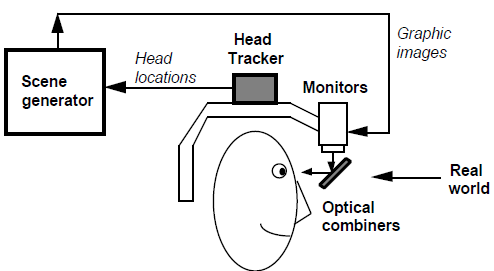
\includegraphics[width=11cm]{./images/see-trough_HMD}
\caption{\label{fig:see-trough_HMD} Diagram \textit{see-trough} HMD}
\end{center}
\end{figure}

\begin{figure}[h]
\begin{center}
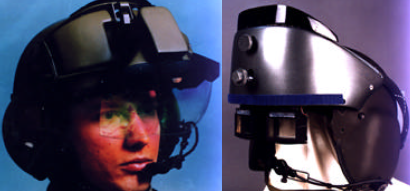
\includegraphics[width=10cm]{./images/actual_see-trough_HMD}
\caption {\label{fig:actual_see_trough_HMD} Contoh \textit{see-through} HMD, dibuat oleh Hughes Electronics}
\end{center}
\end{figure}

\end{itemize}

\subsubsection {\textit{Head-Mounted Projectors}}
\label{subsubsec:HMDP}
\textit{Head-Mounted Projectors} Menggunakan proyektor atau panel LCD kecil dan mempunyai cahaya sendiri untuk menampilkan citra langsung ke lingkungan nyata \cite{Bimber2005}. Seperti yang ditunjukkan oleh gambar \ref{fig:hmpd}.

\begin{figure}[h]
\begin{center}
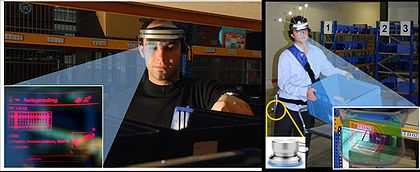
\includegraphics{./images/hmpd}
\caption {\label{fig:hmpd} Ilustrasi penggunaan dua jenis perangkat HMD yang digunakan untuk menampilkan data dan informasi tambahan}
\end{center}
\end{figure}

\subsubsection {\textit{Virtual Retina Display}}
\label{subsubsec:VRD}
\textit{Virtual retina display} (VRD), atau disebut juga dengan \textit{retinal scanning display} (RSD), memproyeksikan cahaya langsung kepada retina mata pengguna\cite{Haller2010}. VRD dapat menampilkan proyeksi citra yang penuh dan juga tembus pandang tergantung pada intensitas cahaya yang dikeluarkan, sehingga pengguna dapat menggabungkan realitas nyata dengan citra yang diproyeksikan  melalui sistem penglihatannya. VRD dapat menampilkan jarak pandang yang lebih luas daripada HMD dengan citra beresolusi tinggi\cite{Jacko2010}.  Keuntungan lain VRD adalah konstruksinya yang kecil dan ringan. Namun, VRD yang ada kini masih merupakan prototipe  yang masih terdapat dalam tahap perkembangan, sehingga masih belum dapat menggantikan HMD yang masih dominan digunakan dalam bidang AR. Gambaran sederhana VRD ini dapat dilihat pada gambar \ref{fig:VRD_diagram}.

\begin{figure}[h!]
	\centering
		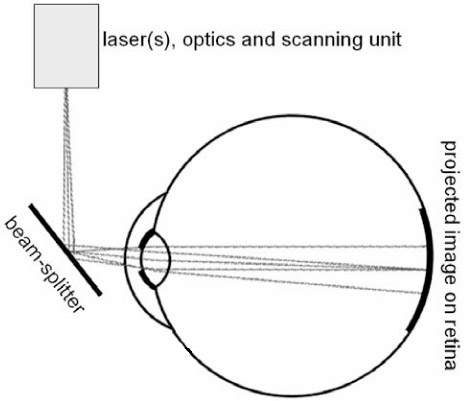
\includegraphics[width=6cm]{images/virtual_retina_diagram}
	\caption{\label{fig:VRD_diagram} Diagram sederhana \textit{virtual retina display}}
\end{figure}

%\begin{figure}[h]
%\begin{center}
%\includegraphics{./images/Vrd_blocks.gif}
%\caption{\label{fig:vrd_block} Diagram Blok \textit{Virtual Retina Display}}
%\end{center}
%\end{figure}

\subsection {\textit{Handheld Display}}
\label{subsec:handheld_display}
Teknik ini menggunakan alat dengan display yang dengan mudah dapat digenggam pengguna (Tablet PC, PDA dan telepon genggam) seperti yang ditunjukkan pada gambar \ref{fig:AR_phone}. Sensor dapat berupa GPS, kompas digital ataupun kamera yang ada pada \textit{handheld} tersebut. Semua penerapan AR pada perangkat genggam menggunakan kamera untuk menggabungkan citra digital dengan lingkungan nyata, \textit{Handheld} AR sangat menjanjikan untuk tujuan komersial. Dua kelebihan utama dari \textit{Handheld} AR adalah mobilitas perangkat yang mudah dan salah satu perangkat genggam yang banyak digunakan (telepon genggam) telah banyak dilengkapi kamera.

\begin{figure}[h!]
	\centering
		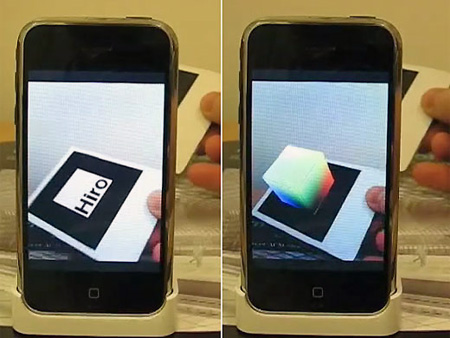
\includegraphics[width=8cm]{images/handphone_AR}
	\caption{\label{fig:AR_phone} Contoh augmented reality dengan \textit{handphone}}
\end{figure}

\subsection {\textit{Spatial Display}}
\label{subsec:spatial_display}
Dalam \textit{Spatial Augmented Reality} (SAR), objek nyata digabungkan langsung dengan citra yang terintegrasi langsung ke lingkungan nyata. Contohnya, citra diproyeksikan ke lingkungan nyata menggunakan proyektor digital atau tergabung dengan lingkungan menggunakan panel display \cite{Ramesh1998}. Perbedaan utama pada SAR dibanding teknik display sebelumnya adalah displaynya terpisah dengan pengguna. SAR memiliki kelebihan dari HMD dan handheld, sistem ini bisa digunakan oleh banyak orang pada waktu bersamaan tanpa perlu mengenakan suatu alat.

Ada tiga teknik display dalam SAR \cite{Bimber2005}, yaitu sebagai berikut:
\begin{enumerate}
\item \textit{Screen-Based Video See-Through Displays}\\
\textit{Screen-based }AR menggabungkan citra dan lingkungan nyata yang ditampilkan ke sebuah monitor, seperti yang ditunjukkan pada gambar \ref{fig:SAR_screen}.

\begin{figure}[h]
	\centering
		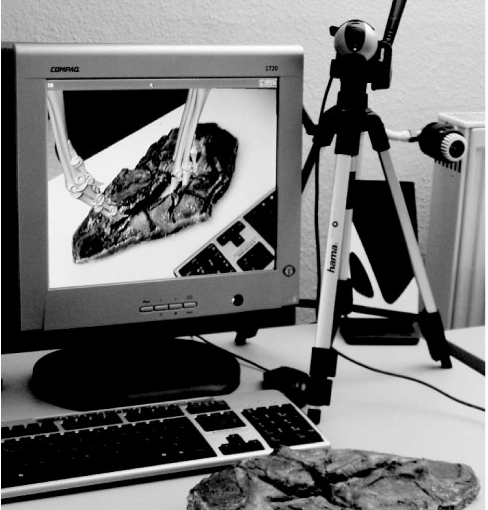
\includegraphics[width=6cm]{images/screen_SAR}
	\caption{\label{fig:SAR_screen} Contoh \textit{Screen-Based Video See-Through Displays} }
\end{figure}

\item \textit{Spatial Optical See-Through Displays}\\
Sistem ini menghasilkan citra yang ditampilkan langsung ke lingkungan nyata. Komponen yang penting dalam sistem ini meliputi \textit{spatial optical combiners} (\textit{planar} atau \textit{curved beam combiners}), layar transparan atau hologram.

\item \textit{Projection-Based Spatial Displays}\\
Sistem ini memproyeksikan citra secara langsung pada permukaan objek fisik daripada menampilkannya pada sebuah bidang pencitraan dalam penglihatan pengguna. Sistem ini menggunakan banyak proyektor yang digunakan untuk meningkatkan wilayah tampilan serta meningkatkan kualitas citra.

\end{enumerate}

\section{Model Tiga Dimensi (3D)}
\label{sec:model_3d}
Pemodelan Tiga Dimensi (3D) (3D \textit{modeling} atau dikenal juga dengan \textit{meshing}) adalah proses pembuatan representasi matematis permukaan tiga dimensi dari suatu objek dengan \textit{software} tertentu. Produk hasil pemodelan itu disebut model 3D. Model 3D tersebut dapat ditampilkan sebagai citra dua dimensi melalui sebuah proses yang disebut \textit{3D rendering}.
%
%Models may be created automatically or manually. The manual modeling process of preparing geometric data for 3D computer graphics is similar to plastic arts such as sculpting.
%
Model 3D direpresentasikan dari kumpulan titik dalam 3D, terhubung oleh berbagai macam entitas geometri, seperti segitiga, garis, permukaan lengkung, dan lain sebagainya. Berdasarkan hal tersebut, model 3D bisa dibuat manual (seperti seni memahat), secara algoritma (pemodelan prosedural), atau \textit{scanning}. Hasil akhir dari citra 3D adalah sekumpulan poligon. Model dengan jumlah poligon yang lebih banyak memerlukan waktu yang lebih lama untuk di-\textit{render} oleh komputer, karena setiap permukaan memiliki tekstur dan \textit{shading} tersendiri. 

\section{Aplikasi Komputer Berbasis Web (\textit{Rich Internet Application})}
\label{sec:aplikasi_web}

Pada tahun 90-an, "mengakses \textit{web}" berarti mengakses tulisan dan gambar statis secara \textit{online} . Sejalan dengan berkembangnya koneksi internet, kebutuhan akan suatu konten yang lebih kaya, responsif juga meningkat. Pada tahun 2002, Macromedia menemukan istilah \textit{Rich Internet applications} (RIAs). RIAs menggabungkan fleksibilitas, tingkat responsif, dan kemudahan aplikasi berbasis desktop. RIAs atau dikenal dengan aplikasi berbasis \textit{web} adalah aplikasi yang mempunyai karakteristik seperti aplikasi \textit{desktop}, biasanya didistribusikan atau diakses lewat \textit{browser web} standar, menggunakan \textit{web plug-in}. Contoh RIAs meliputi Ajax, Curl, GWT, Adobe Flash/Adobe Flex/AIR, Java/JavaFX, Mozilla's XUL dan Microsoft Silverlight. 

Aplikasi berbasis \textit{web} semakin banyak dikembangkan, karena kelebihan aplikasi \textit{web} yang sangat baik untuk aplikasi dengan model \textit{client-server}. Beberapa kelebihan aplikasi \textit{web} dibanding aplikasi \textit{desktop}:
\begin{enumerate}
	\item \textit{Running anywhere} (berjalan/beroperasi dimana saja), cukup instalasi pada satu \textit{server} dan tanpa perlu instalasi apapun selama ada \textit{web browser} di sisi \textit{client}, pengguna langsung  dapat menjalankan aplikasi tersebut tanpa konfigurasi apapun. Secara default, \textit{web browser} pada sistem operasi apapun telah tersedia sehingga kebutuhan akan \textit{web browser} untuk menjalankan aplikasi bukanlah suatu kendala berarti.
	\item \textit{Easy to update} (mudah untuk diubah/diperbaharui), cukup \textit{update} pada sisi \textit{server} maka aplikasi pada \textit{client} akan langsung menggunakan versi ter-\textit{update} tanpa harus instalasi dulu pada \textit{client}.
	\item \textit{Requirement} (kebutuhan)pada \textit{client} tidak terlalu besar. Karena \textit{running} aplikasi bersifat \textit{stateless} dan pada sisi \textit{client} hanya sebagai \textit{interface} maka spesifikasi hardware pada \textit{client} tidak harus canggih. 
	\item Tampilan yang lebih beragam.
\end{enumerate} 

\section {Adobe Flash \textit{Platform}}
\label{subsec:adobe_flash_platform}
Kebanyakan \textit{designer} dan \textit{developer} menggunakan Adobe Flash ataupun Adobe Flex, yang merupakan bagian dari platform Adobe Flash, untuk mengembangkan RIAs. Flash merupakan suatu \textit{environment} untuk membuat konten yang interaktif dan kaya fitur dalam dunia \textit{web}. Begitu juga Flex merupakan sebuah \textit{framework} \textit{cross-platform} untuk mengembangkan RIAs. Konten yang dibuat dengan Flash dan Flex di-\textit{deploy} menggunakan Adobe Flash Player

\subsection {Adobe Flash}
\label{subsec:adobe_flash}
Adobe Flash (dulunya Macromedia Flash) adalah platform multimedia yang aslinya dibuat oleh Macromedia dan saat ini dikembangkan dan didistribusikan oleh Adobe Systems. Sejak pengenalannya pada Tahun 1996, Flash telah menjadi metode yang popular untuk menambahkan animasi dan interaktivitas ke halaman web. Komponen Flash untuk mengintegrasikan video ke halaman web, dan yang terbaru saat ini, untuk mengembangkan RIAs.

Flash dapat memanipulasi vector dan raster grafik, serta mendukung \textit{streaming} dua arah audio dan video. Flash menggunakan bahasa \textit{script} yang disebut Action Script. Banyak produk \textit{software}, sistem dan \textit{device} dapat menampilkan konten flash, contohnya Adobe Flash player, yang tersedia gratis bagi sebagian besar \textit{web browser}. Beberapa ponsel dan alat elektronik lainnya juga dapat menampilkan konten Flash, menggunakan Flash lite.

\textit{File} dalam format SWF, biasanya disebut "ShockWave Flash movies", "Flash movies" atau "Flash games", yang biasanya memiliki sebuah ekstensi .swf dan dapat menjadi objek di halaman \textit{web}. \textit{File} tersebut pada dasarnya dijalankan dengan Flash Player itu sendiri atau digabungkan dengan "Projector" (\textit{video flash} yang dapat berjalan sendiri dengan ekstensi .exe di Microsoft Windows atau .hqx untuk Macintosh). \textit{File} Flash Video memiliki ekstensi .flv dan juga digunakan dalam .swf atau dijalankan melalui aplikasi yang dapat menjalankan \textit{file} flv.

\subsection {Adobe Flex}
\label{subsec:adobe_flex}
Adobe Flex adalah paket pengembangan \textit{software} yang dirilis oleh Adobe systems untuk pengembangan dan aplikasi \textit{cross-platform rich internet} berbasis platform adobe flash. Aplikasi flex dapat ditulis menggunakan Adobe Flash Builder sebagai IDE (\textit{Integrated Development Evironment}) dan menggunakan Flex \textit{Software Development Kit} (SDK) yang tersedia gratis dari Adobe. 

Flex membuat \textit{workflow} dan model pemrograman yang familiar terhadap \textit{developer} aplikasi berbasis \textit{web}. FLex menggunakan MXML dan ActionScript. MXML merupakan sebuah bahasa yang berbasis XML, menawarkan cara membangun dan menata \textit{user interface}. Interaktivitas dicapai melalui penggunaan ActionScript, yaitu bahasa utama Flash Player.

Flex menyediakan dua kompiler: mxmlc dan compc. Kompiler compc dan mxmlc bisa dijalankan dari Flex Builder atau pun dari \textit{command line}. compc digunakan untuk mengkompilasi komponen, kelas, and file lainnya ke file SWC atau RSL yang digunakan sebagai \textit{library} untuk aplikasi. mxmlc untuk mengkompilasi ActionScript dan SWC ke \textit{file} SWF, seperti ditunjukkan pada gambar \ref{fig:compile_flex}. Setelah aplikasi dikompilasi dan di-\textit{deploy} ke \textit{web server}, pengguna bisa mengakses file SWF tersebut dan dijalankan via \textit{web browser}.

\begin{figure}
\begin{center}
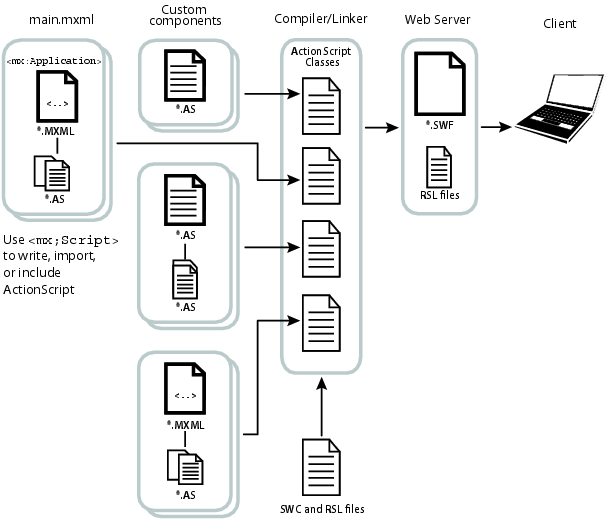
\includegraphics[width=9cm]{./images/compile_flex.png}
\caption{\label{fig:compile_flex} Diagram Kompilasi Flex}
\end{center}
\end{figure}

\subsection {ActionScript}
\label{subsec:action_script}
ActionScript merupakan bahasa pemrograman berorientasi objek yang berdasarkan ECMAScript (bahasa yang distandarisasi oleh Ecma International dalam spesifikasi ECMA-262 dan ISO/IEC 16262). ActionScript  terutama digunakan untuk pengembangan \textit{website} dan \textit{software} menggunakan Adobe Flash Player (dalam bentuk \textit{file} SWF yang diintegrasikan  ke halaman \textit{web}), ActionScript juga digunakan pada beberapa aplikasi untuk \textit{database}  (seperti Alpha Five). ActionScript pada awalnya didesain untuk mengatur animasi vektor 2D sederhana yang dibuat di Adobe Flash, dengan berkembangnya. Versi terakhir dari ActionScript menambahkan kemungkinan penggunaan  untuk pembuatan \textit{web} berbasis \textit{game} dan RIAs dengan media \textit{streaming} (seperti video dan audio).

\section{\textit{Library} Pendukung Augmented Reality Pada Platform Flash}
\label {sec:library_AR}
\textit{Library} atau Pustaka, dalam ilmu komputer adalah koleksi dari rutin-rutin program yang digunakan untuk membangun dan mengembangkan \textit{software}. \textit{Library}, umumnya mengandung kode program dan data pembantu (banyak \textit{programmer} menyebutnya sebagai \textit{helper}), yang menyediakan layanan-layanan kepada program-program independen. Penggunaan \textit{library} sangat diperlukan untuk mengembangkan aplikasi AR secara cepat. \textit{Library} AR yang dikenal luas dalam platform Flash adalah FLARToolKit.

\subsection {FLARToolKit}
\label {subsec:FLARToolKit}
%\subsection {FLARToolKit}
%\label{subsec:FLARToolKit}
%Pada bulan november 2008, sebuah grup pemrograman di Jepang, mengembangkan banyak proyek dengan ActionScript sehingga memberi ide kepada para \textit{developer} akan apa yang bisa dilakukan bahasa tersebut. FLARToolKit, pertama kali dikembangkan oleh Tomohiko Koyama (aka Saqoosha), ia mengenalkan AR ke dunia \textit{web}, dan ke segmen pengguna yang lebih luas.

FLARToolKit adalah \textit{tracking system library} yang bersifat \textit{open-source} sehingga memungkinkan \textit{programmer} dengan mudah mengembangkan aplikasi AR, FLARToolKit merupakan \textit{porting} (perubahan terhadap \textit{software} untuk menjadikannya dapat digunakan di lingkungan yang berbeda) yang paling terakhir dari ARToolkit, yaitu sebuah libary AR C++ yang awalnya dikembangkan oleh Dr. Hirokazu Kato di  Human Interface Technology Lab University of Washington. Dengan datangnya ActionScript 3.0, para pengembang seperti Mario Klingemann dan lainnya mulai bereksperimen dengan teknik analisis image secara \textit{real-time} untuk  Flash Player. Saqoosha meneruskan hal ini, dan mem-\textit{porting} FLARToolKit dari NYARToolkit (sebuah Java/C-sharp/Android \textit{port} dari ARToolkit).

FLARToolKit hanya merupakan \textit{library} untuk \textit{tracking} pada AR, untuk menampilkan objek 3D di lingkungan Flash, FLARToolKit memerlukan sebuah \textit{library} 3D. Beberapa \textit{library} 3D yang didukung oleh FLARToolKit adalah sebagai berikut:
\begin{itemize}
\item Alternativa3D
\item Away3D
\item Away3D Lite
\item Papervision3D
\item Sandy3D
\end{itemize}

Proses FLARToolKit secara garis besarnya sebagai berikut: 

\begin{enumerate}
	\item Mengambil video dari \textit{webcam}.
	\item Binarisasi citra masukan(\textit{thresholding}).
	\item Memberi penanda (\textit{labelling}).
	\item Deteksi area persegi (\textit{Marker Outline Detection}). 
	\item Pencocokan pola.
	\item Menghitung transform matrix.
	\item Merender obyek 3D.
\end{enumerate}

\subsubsection {Mengambil Video dari \textit{Webcam}}
\label{subsubsec:capture_webcam}
Langkah awal yang harus dilakukan adalah mendapatkan masukan video dari sebuah \textit{webcam}, seperti yang ditunjukkan gambar \ref{fig:capture_from_webcam}. Video yang di-\textit{streaming} secara \textit{real-time} ini akan diolah oleh sistem untuk dianalisa \textit{frame} per \textit{frame}. Sebelum \textit{webcam} digunakan, \textit{webcam} harus dikaliberasi terlebih dahulu. Kaliberasi \textit{webcam} merupakan bagian yang sangat penting dalam proses pengambilan masukan video. Hal ini disebabkan oleh distorsi pada lensa \textit{webcam} yang tiap-tiap kamera berbeda karakteristiknya (gambar \ref{fig:distorted_image}). Tujuan dari kalibrasi \textit{webcam} adalah untuk menghitung tingkat distorsi dari sebuah lensa \textit{webcam} yang digunakan agar citra yang dihasilkan mendekati citra ideal.

\begin{figure}[h]
\begin{center}
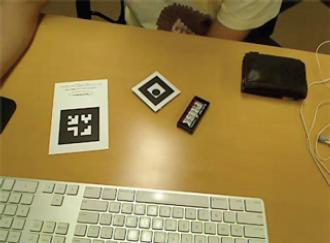
\includegraphics[width=7cm]{./images/flartk/capture_webcam.JPG}
\caption{\label{fig:capture_from_webcam} Mengambil citra dari \textit{webcam}}
\end{center}
\end{figure}

%Menggunakan \textit{class} kamera dan video kemudian menggambar video contohnya ke BitmapData. 

\begin{figure}[h]
\begin{center}
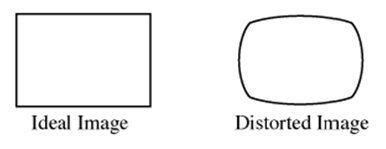
\includegraphics[width=6cm]{./images/flartk/distorted_image.JPG}
\caption{\label{fig:distorted_image} Perbandingan antara citra yang ideal dengan citra yang disebabkan oleh faktor distorsi}
\end{center}
\end{figure}

\subsubsection {Binarisasi Citra Masukan (\textit{Thresholding})}
\label{subsubsec:thresholding}
Langkah pertama pada aplikasi visi komputer yang terletak pada deteksi tepi adalah untuk men-\textit{threshold} sumber citra atau disebut juga binarisasi seperti yang ditunjukkan gambar \ref{fig:thresholding}. \textit{Thresholding} mengkonversi citra ke citra binari sehingga memudahkan untuk komputasi. Sebuah citra binari dibuat dengan mengubah pixel yang lebih cerah daripada nilai \textit{threshold} ke suatu warna, dan pixel yang lebih gelap daripada nilai \textit{threshold} ke suatu warna lainnya (didefinisikan sebagai \textit{gray-scale} atau hitam-putih). Nilai \textit{threshold} berada pada angka 0 – 255 dan secara default, \textit{threshold} bernilai 100. Fungsi dari proses ini adalah untuk membantu sistem agar dapat mengenali bentuk segi empat dan pola di marker pada citra yang diterima. Nilai \textit{threshold} dapat dirubah dan disesuaikan dengan kondisi cahaya disekitar \textit{marker} untuk tetap membuat \textit{marker} terlihat sebagai segi empat, karena ketika cahaya disekitar \textit{marker} berkurang ataupun berlebih pada saat proses \textit{thresholding}, sistem tidak dapat mendeteksi \textit{marker}.
%\begin{figure}[h]
%\begin{center}
%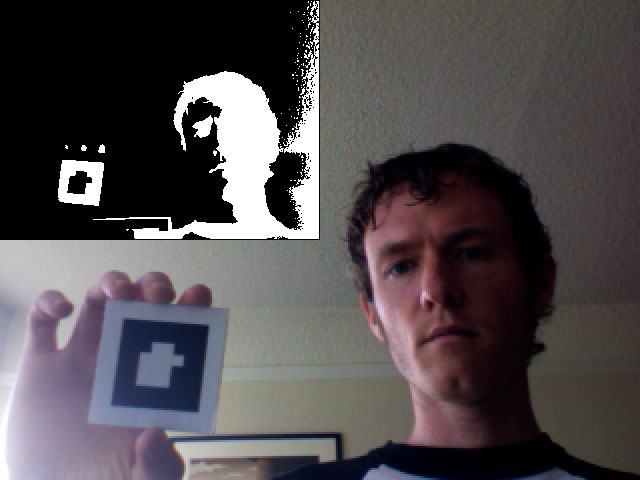
\includegraphics[width=7cm]{./images/thresholding}
%\caption{\label{fig:thresholding} Thresholding}
%\end{center}
%\end{figure}
\begin{figure}
\begin{center}
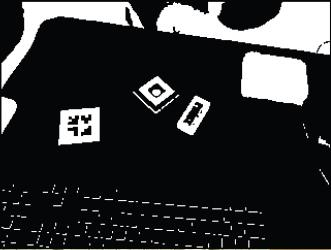
\includegraphics[width=7cm]{./images/flartk/binarize.JPG}
\caption{\label{fig:thresholding} Thresholding}
\end{center}
\end{figure}

\subsubsection {Memberi Penanda (\textit{Labeling})}
\label{subsubsec:labeling}
Langkah berikutnya dari FLARToolKit adalah menemukan area yang berdampingan dalam citra yang di-\textit{treshold}, khususnya dalam area dibawah \textit{threshold} (area yang lebih gelap). Area yang berdampingan diberi tanda dengan warna yang berbeda dengan tujuan untuk mengidentifikasi area, proses \textit{labelling} dapat dilihat pada gambar \ref{fig:labelling}.
%Dengan menggunakan fungsi \textit{BitmapData.getColorBoundsRect} dan \textit{BitmapData.foodFill}, 

\begin{figure}[h]
\begin{center}
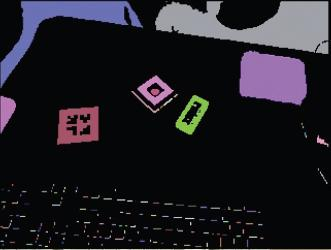
\includegraphics[width=7cm]{./images/flartk/labelling.JPG}
\caption{\label{fig:labelling} Setiap area putih ditandai dengan warna yang berbeda.}
\end{center}
\end{figure}

\subsubsection {Deteksi Area Persegi (\textit{Marker Outline Detection})}
\label{subsubsec:outline_detection}
Langkah selanjutnya, FLARToolKit mencari area yang kemudian ditandai sebagai persegi \textit{(marker outline)}. Setelah citra mengalami proses \textit{thresholding} dan \textit{labelling}, FLARToolkit akan mengenali bentuk dan pola yang ada pada marker. FLARToolkit akan mencari bagian yang memiliki bentuk segi empat dan menandainya. FLARToolKit juga akan menghilangkan area yang tidak berbentuk segi empat sehingga yang akan ditampilkan pada layar hanyalah area yang memiliki bentuk segi empat (gambar \ref{fig:find_squares}.
%With candidates for marker locations, FLARToolKit then proceeds to search the labeled areas for shapes that could be transformed squares (i.e. marker outlines).

\begin{figure}[h]
\begin{center}
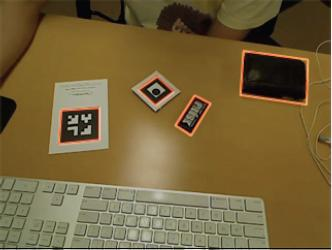
\includegraphics[width=7cm]{./images/flartk/find_squares.JPG}
\caption{\label{fig:find_squares} Mencari area persegi (Marker Outline Detection)}
\end{center}
\end{figure} 

\subsubsection {Pencocokan Pola}
\label{subsubsec:pattern_matching}
Setelah semua area persegi ditandai, FLARToolKit menganalisa citra yang berada di dalam persegi dan membandingkan polanya dengan sekumpulan pola yang telah ditentukan (pencocokan pola). FLARToolKit mengekstrak pola di dalam persegi menggunakan transformasi \textit{homography}. FLARToolKit memberikan sebuah nilai '\textit{confidence}' kepada setiap pola yang cocok, jika kecocokannya di atas nilai yang telah ditentukan maka polanya dinyatakan cocok. 

\begin{figure}
\begin{center}
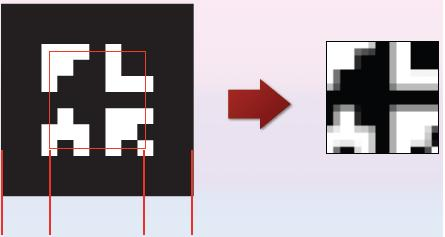
\includegraphics[width=7cm]{./images/flartk/marker_spec.JPG}
\caption{\label{fig:marker_spec} Spesifikasi pola marker}
\end{center}
\end{figure} 

Spesifikasi pola marker (gambar \ref{fig:marker_spec}):
\begin{itemize}
	\item Harus berupa persegi.
	\item Hanya 50\% dari tengah area yang digunakan untuk proses pencocokan pola.
	\item Pola marker secara \textit{default}-nya adalah 16 x 16 titik.
	\item Ukuran pola bisa lebih besar, tapi membutuhkan waktu yang lebih lama untuk diproses.
\end{itemize}

%\begin{figure}[h!]
%	\begin{center}
%		\subfloat {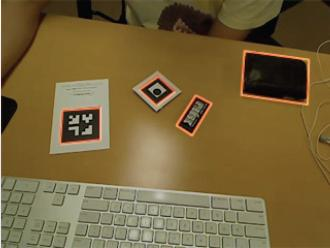
\includegraphics[width=5cm]{./images/flartk/matching_pattern.JPG} \label{fig:pattern_matching1}}\\
%		\subfloat {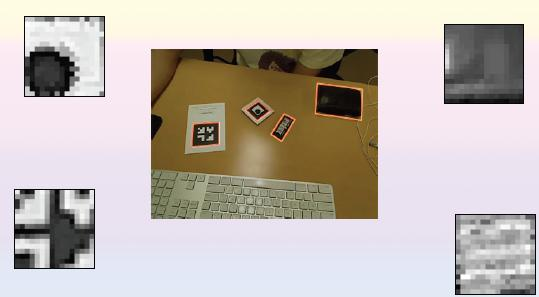
\includegraphics[width=5cm]{./images/flartk/matching_pattern2.JPG} \label{fig:pattern_matching2}}\\
%		\subfloat {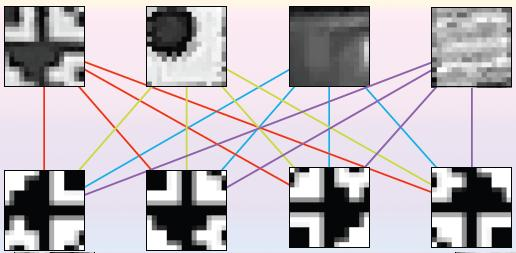
\includegraphics[width=5cm]{./images/flartk/matching_pattern3.JPG} \label{fig:pattern_matching3}}\\
%		\subfloat {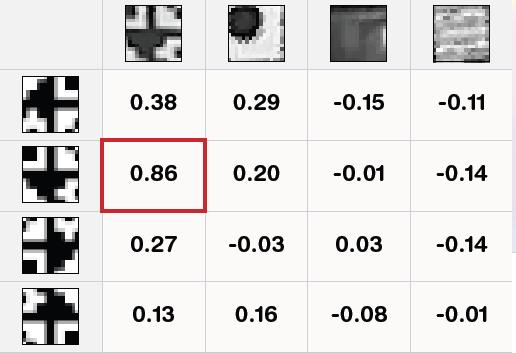
\includegraphics[width=5cm]{./images/flartk/matching_pattern4.JPG} \label{fig:pattern_matching4}}
%		\caption {\label{fig:pattern_matching} Proses pencocokan pola}
%	\end{center}
%\end{figure}

\subsubsection {Menghitung Transformasi Matriks}
\label{subsubsec:calculate_transform_matrix}
Transformasi matriks dihitung dari titik-titik persegi marker yang dideteksi. Matriks tersebut digunakan untuk proses \textit{render} objek 3D.% Algoritmanya dapat dilihat dalam paper di http://www.hitl.washington.edu/artoolkit/publications/.
%
%\begin{figure}[h!]
%\begin{center}
%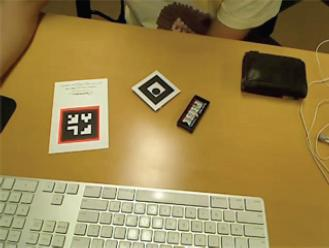
\includegraphics[width=7cm]{./images/flartk/calculate_transform_matrix.JPG}
%\caption{\label{fig:calculate_matrix} Kalkulasi transformasi matriks}
%\end{center}
%\end{figure} 

\subsubsection {Me-\textit{render} Objek 3D}
\label{subsubsec:render_the_3d_objects}
FLARToolKit menggunakan transformasi matriks yang dikalkulasikan di step sebelumnya dan menampilkan objek yang sesuai dengan sebuah \textit{library} 3D, seperti yang ditunjukkan gambar \ref{fig:render_3d_objects}. FLARToolKit menyertakan kelas pendukung yang mengkonversikan transformasi matriks FLARTollKit ke setiap kelas matriks internal \textit{library} 3D tersebut.

\begin{figure}[h!]
\begin{center}
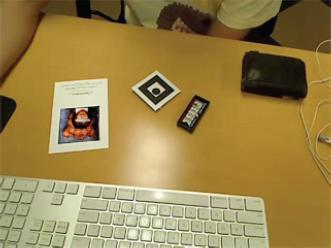
\includegraphics[width=7cm]{./images/flartk/render_3d_objects.JPG}
\caption{\label{fig:render_3d_objects} Render objek 3D}
\end{center}
\end{figure} 

\subsection {Papervision3D}
\label{subsec:Papervision3D}
Salah satu \textit{library} 3D (biasa disebut juga dengan \textit{engine} 3D) untuk platform Flash adalah Papervision3D, Papervison3D merupakan \textit{library} 3D yang bersifat \textit{open source}. Dengan Papervision 3D, model 3D bisa dibuat di platform Flash menggunakan kelas-kelas dalam ActionScript ataupun juga dengan meng-\textit{import} model yang dibuat dari \textit{software} pemodelan 3D. Model yang telah dibuat atau di-\textit{import}, bisa dikendalikan dengan ActionScript.

\subsection {FLARManager}
\label{subsec:FLARManager}
Visi komputer dalam konteks \textit{web} memiliki banyak kesulitan untuk diterapkan. Masalah utama ialah kurangnya kendali terhadap kondisi lingkungan \textit{end-user}. Kurangnya atau ketidakteraturan pencahayaan membuat analisis dari sebuah citra sangat sulit, dan permasalahan tersebut berdampak pada FLARToolKit. Selain itu, FLARToolKit sangat sulit digunakan karena minimnya dokumentasi, dan \textit{developer} harus membuat sebuah \textit{manager} untuk mengatur konfigurasi kamera, marker dan juga objek virtual yang akan ditampilkan. 

FLARManager adalah sebuah \textit{framework} sederhana yang memudahkan untuk membuat aplikasi AR dengan Flash terutama yang menggunakan \textit{libray} FLARToolKit. \textit{Framework} merupakan kumpulan komponen kelas sekaligus kerangka dalam pemrograman yang memudahkan \textit{programmer} untuk membuat suatu aplikasi yang siap pakai. FLARManager bisa meningkatkan akurasi dan reabilitas dari proses dengan hanya merubah konfigurasinya yang berupa file dengan format xml. FLARManager dapat mendeteksi lebih dari satu \textit{marker} dan pola dalam waktu bersamaan, sehingga bisa menampilkan objek virtual lebih dari satu.

FLARToolkit menyediakan akses ke sumber citra yang diprosesnya, dan juga hasil dari FLARToolkit setelah di analisa. Dengan demikian, FLARManager bisa difokuskan pada fungsionalitas dalam deteksi dan \textit{tracking} dari \textit{marker}. FLARManager sebisa mungkin menghindari perubahan terhadap FLARToolkit. Dengan tidak tergantungnya FLARManager terhadap FLARToolkit, setiap proyek bisa terus dikembangkan secara terpisah, dan FLARManager secara teori bisa diterapkan pada \textit{libray} Flash AR lainnya.

Sampai saat tulisan ini dibuat, FLARManager telah mendukung \textit{tracking library} sebagai berikut :
\begin{itemize}
\item FLARToolkit
\item flare*tracker
\item flare*NFT
\end{itemize}

